\documentclass[a4paper, 12pt]{article}%тип документа

%отступы
\usepackage[left=2cm,right=2cm,top=2cm,bottom=3cm,bindingoffset=0cm]{geometry}

%Русский язык
\usepackage[T2A]{fontenc} %кодировка
\usepackage[utf8]{inputenc} %кодировка исходного кода
\usepackage[english,russian]{babel} %локализация и переносы

%Вставка картинок
\usepackage{wrapfig}
\usepackage{graphicx}
\graphicspath{{pictures/}}
\DeclareGraphicsExtensions{.pdf,.png,.jpg}

%Графики
\usepackage{multirow}
\usepackage{pgfplots}
\pgfplotsset{compat=1.9}

%Математика
\usepackage{amsmath, amsfonts, amssymb, amsthm, mathtools}

%Заголовок
\author{Сифат Мд Абдуллах Ал Хасиб \\
Физтех школа электроники, фотоники и молекулярной физики \\
Группа Б04-105}
\title{\textbf{Лаборатория Работа 2.1.1 \\ 
Измерение удельной теплоёмкости воздуха при постоянном давлении}}
\begin{document}
\maketitle 
\section{Введение}\textbf{Цель работы}: измерить повышение температуры воздуха в зависимости от мощности подводимого тепла и расхода при стационарном течении через трубу; 
2) исключив тепловые потери, по результатам измерений определить теплоёмкость воздуха при постоянном давлении.\\
\textbf{В работе используются}: теплоизолированная стеклянная трубка; электронагреватель; источник питания постоянного тока; амперметр; вольтметр (цифровые мультиметры); термопара, подключённая к микровольтметру; компрессор; газовый счётчик; секундомер.
\section{Теоретическая справка}
Измерение теплоёмкости тел обычно производится в калориметрах, т.е. в сосудах, обеспечивающих теплоизоляцию исследуемого тела от внешней среды. При этом регистрируется изменение его температуры $\delta T$ в зависимости от количества тепла $\delta Q$, полученного телом от некоторого нагревательного элемента внутри калориметра. Теплоёмкость тела в некотором процессе определяется как их отношение:
\begin{equation}
\begin{aligned}
C = \dfrac{\delta Q}{\delta T} 
\end{aligned}
\end{equation}
Надёжность измерения определяется, в основном, качеством калориметра. Необходимо, чтобы количество тепла, затрачиваемое на нагревание исследуемого тела, существенно превосходило тепло, расходуемое на нагревание самого калориметра, а также на потери тепла из установки. При измерении теплоёмкости газов эти требования выполнить довольно трудно - масса газа в калориметре и, следовательно, количество тепла, идущее на его нагревание, как правило, малы. Для увеличения количества нагреваемого газа при неизменных размерах установки в нашей работе исследуемый газ (воздух) продувается через калориметр, внутри которого установлен нагреватель. При этом измеряются мощность нагревателя, масса воздуха, протекающего в единицу времени (расход), и приращение его температуры.
\newpage
\begin{wrapfigure}{r}{0.6\textwidth}
  \begin{center}
    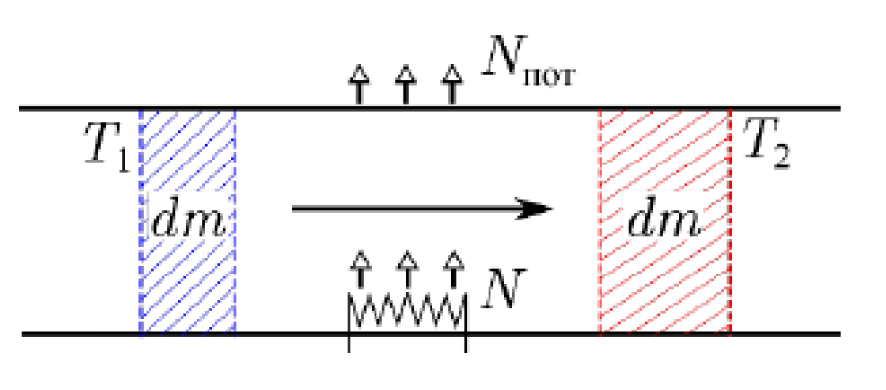
\includegraphics[width = 0.6\textwidth]{Fig.1.png}
  \end{center}
  \textbf{\caption{Нагрев газа при течении по трубе}}
\end{wrapfigure}
Рассмотрим газ, протекающий стационарно слева направо через трубу постоянного сечения, в кото-рой установлен нагревательный элемент (см.рис.1). Пусть за некоторое время $dt$ через калориметр прошла малая порция газа массой $dm = q dt$ , где $q$ [кг/с] - массовый расход газа в трубе. Если мощность нагрева равна $N$, мощность тепловых потерь на обмен с окружающей средой $N_{\text{пот}}$, то порция получила тепло $\delta Q =(N - N_{\text{пот}})dt$. С другой стороны, по определению теплоёмкости
(1): $\delta Q =c dm \Delta T$ , где $\Delta T = T_2 - T_1$ - приращение температуры газа, и $c$ — удельная (на единицу массы) теплоёмкость газа в рассматриваемом процессе. При малых расходах газа и достаточно большом диаметре трубы перепад давления на её концах мал, поэтому можно принять, что $P_1 \approx P_2 = P_0$, где $P_0$ - атмосферное давление. Следовательно, в условиях опыта измеряется удельная теплоёмкость при постоянном давлении $c_P$. Таким образом, получаем
\begin{equation}
\begin{aligned}
C_p = \dfrac{N - N_{\text{пот}}}{q \Delta T} 
\end{aligned}
\end{equation}
\section{Экспериментальная установка}
Схема установки изображена на рис. 1. Воздух, нагнетаемый компрессором, прокачивается через калориметр. Калориметр представляет собой стеклянную цилиндрическую трубку с двойными стенками, запаянными с торцов. На внутреннюю поверхность стенок трубки нанесено серебряное покрытие для минимизации потерь тепла за счет излучения. Воздух из пространства между стенками калориметра откачан до высокого вакуума ($10^{-5}$ торр) для минимизации потерь тепла, обусловленных теплопроводностью.
\begin{center}
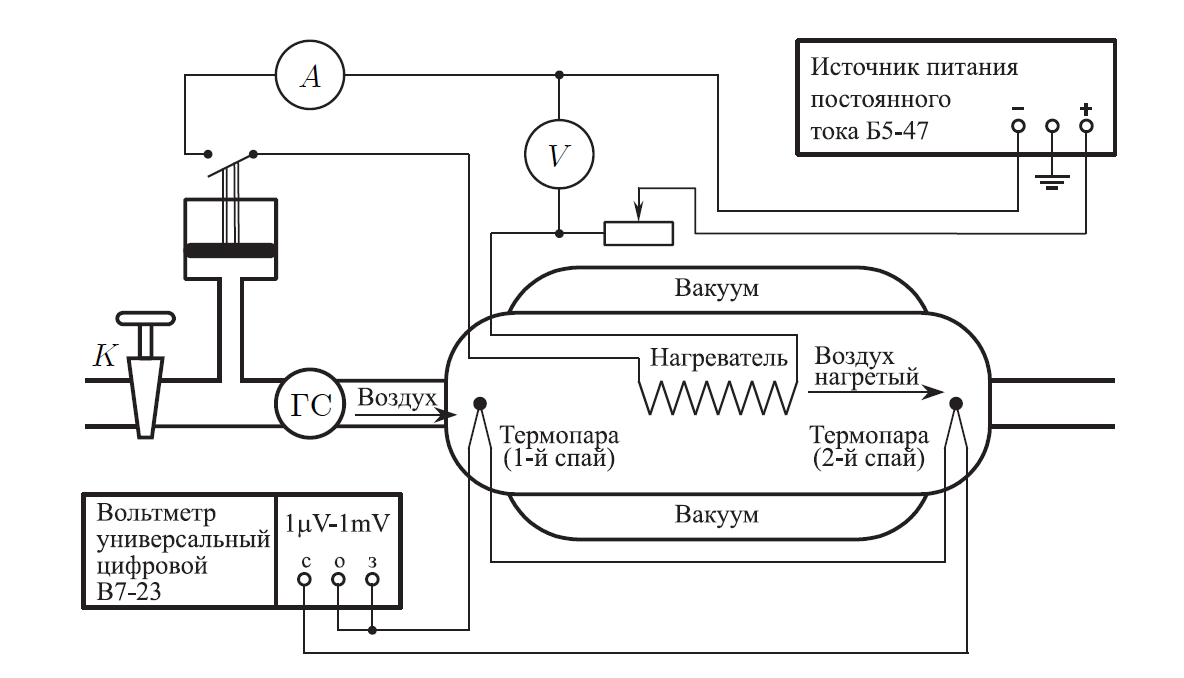
\includegraphics[width = 0.8\textwidth]{Fig.2.png}
\end{center}
Нагреватель в виде намотанной на пенопласт нихромовой проволоки раcположен внутри калориметра непосредственно в воздушном потоке. Нагрев проволоки производится от регулируемого источника постоянного тока (ИП). Напряжение $U$ на нагревателе и ток $I$ через него регистрируются цифровыми мультиметрами. Таким образом, мощность нагрева равна
\begin{equation}
\begin{aligned}
N = UI 
\end{aligned}
\end{equation}
Для измерения разности температур $\Delta T$ служит медно-константановая термопара. Один спай термопары расположен в струе воздуха, входящего в калориметр, и находится при комнатной температуре, а второй - в струе выходящего нагретого воздуха. Константановая проволока термопары расположена внутри калориметра, а медные проводники подключены к цифровому вольтметру. Возникающая в термопаре ЭДС $\varepsilon$ пропорциональна разности температур $\Delta T$ спаев:
\begin{equation}
\begin{aligned}
\varepsilon = \beta \Delta T
\end{aligned}
\end{equation}
где $\beta = 40,7 \dfrac{\text{мкВ}}{ ^{\circ} C}$ - чувствительность медно-константановой термопары в рабочем диапазоне температур (20-30 $ ^{\circ} C$). ЭДС регистрируется с помощью микровольтметра.

Объём воздуха, прошедшего через калориметр, измеряется газовым счётчиком ГС. Для регулировки расхода служит кран К. Время $\Delta t$ прохождения некоторого объема $\Delta V$ воздуха измеряется секундомером. Объёмный расход равен $\Delta V / \Delta t$, массовый расход может быть найден как
\begin{equation}
\begin{aligned}
q = \rho_0 \dfrac{\Delta V}{\Delta t} 
\end{aligned}
\end{equation}
где $\rho_0$ - плотность воздуха при комнатной температуре, которая в свою очередь может быть получена из уравнения Менделеева–Клапейрона: $\rho_0 = \dfrac{\mu P_0}{RT_0}$, где $P_0$ - атмосферное давление, $T_0$ - комнатная температура (в Кельвинах), $\mu$ = 29,0 г/моль - средняя молярная масса (сухого) воздуха.

Учитывая особенности устройства калориметра, следует ожидать, что мощность нагревателя расходуется не только на нагрев массы прокачиваемого воздуха, но и частично теряется за счет нагрева внутренних стенок термостата и рассеяния тепла через торцы термостата. Можно предположить, что при небольшом нагреве ($\Delta T << T_0$) мощность потерь тепла $N_{\text{пот}}$ прямо пропорциональна разности температур:
\begin{equation}
\begin{aligned}
N_{\text{пот}} = \alpha \Delta T
\end{aligned}
\end{equation}
где $\alpha$ — некоторая константа. При этом условии основное соотношение (2) принимает вид
\begin{equation}
\begin{aligned}
N = (c_p q+ \alpha) \Delta T
\end{aligned}
\end{equation}
Следовательно, при фиксированном расходе воздуха ($q = const$) подводимая мощность и разность температур связаны прямой пропорциональностью ($\Delta T (N)$ — линейная функция).
\section{Ход работы}
\begin{center}

\begin{tabular}{|c|c|c|c|c|c|}
\hline $P_0,\ \text{мм}.\ \text{рт}.\ \text{ст}. $ & $T_{\text{к}}, \text{K}$ & $\varphi, \%$ & $\Delta t_{max}, c$ & $\Delta V_{max},\ \text{дм}^3$ & $P_{\text{н.п.}},\ \text{кПа}$ \\\hline
 $749.5 \pm 0.5$ & $294 \pm 1$ & $81 \pm 1$ & $26.0 \pm 0.5$ & $5 \pm 0.1$ & $2.48$ \\\hline
\end{tabular}
\end{center}
Объёмный расход для каждого из опытов вычислим по формуле:
\[
	q = \rho_0 \frac{\Delta V}{\Delta t}
\]
\[
	\rho_0 = \frac{\mu \left(P_0 - \varphi P_{\text{н. п.}} \right)}{RT_\text{к}} = 1.18 \pm 0.01\ \frac{\text{кг}}{\text{м}^3};
\]
\[
	\sigma
\]

\begin{center}

\begin{tabular}{|c|c|c|c|c|c|}
\hline $\Delta t_1, c$ & $\Delta V_1, \text{дм}^3$ & $q_1, \frac{\text{г}}{c}$ & $\Delta t_2, c$ & $\Delta V_2, \text{дм}^3$ & $q_2, \frac{\text{г}}{c}$ \\\hline
 $26.0 \pm 0.5$ & $5 \pm 0.1$ & $0.2 \pm 0.03$ & $44.8 \pm 0.5$ & $5 \pm 0.1$ & $0.135 \pm 0.03$ \\\hline
\end{tabular}
\end{center}

Посчитаем мощность нагрева $N$ и разность температур $\Delta T$ по формулам:
\[
	N = UI;
\]
\[
	\Delta T = \frac{\mathcal{E}}{\beta}.
\]
При расходе $q_1$:



\begin{center}
\begin{tabular}{|c|c|c|c|c|c|c|c|}\hline
{} &   $\mathcal{E}, \text{мкВ}$ & $U_\text{н}, \text{В}$ & $I_\text{н}, \text{мА}$ & $\Delta t, K$ & $N,\, \text{Вт}$ & $R_\text{н},\ \text{Ом}$ \\\hline
1 &   67 &  3.58 &  120.7 &  1.91 &   0.43 & 35 \\\hline
2 &   86 &  4.03 &  136.69 & 2.45 &   0.55 &  35.4 \\\hline
3 &  99 &  4.53 &  153.37 &  2.83 &  0.69 &  35.3 \\\hline
4 &  120 &  5.05 & 170.68 &  3.42 &  0.86 &  35.3 \\\hline
5 &  149 &  5.525 & 187.31 & 4.26 &  1.03 &  35.3 \\\hline
6 &  178 &  5.980 & 210.10 & 5.09 &  1.26 &  35.3 \\\hline
\end{tabular}
\end{center}
При расходе $q_2$:
\begin{center}

\begin{tabular}{|c|c|c|c|c|c|c|c|}\hline
{} &   $\mathcal{E}, \text{мкВ}$ & $U_\text{н}, \text{В}$ & $I_\text{н}, \text{мА}$ & $\Delta t, K$ & $N,\, \text{Вт}$ & $R_\text{н},\ \text{Ом}$ \\\hline
1 &   48 &  3.479 &   118.26 &  1.37 &  0.41 &  35.6 \\\hline
2 &   89 &  4.005 &  136.16 &  2.54 &  0.54 &  35.3 \\\hline
3 &  114 &  4.531 &  153.97 &  3.26 &  0.69 &  35.3 \\\hline
4 &  155 &  5.033 &  170.85 &  4.42 &  0.859 & 35.3 \\\hline
5 &  188 &  5.39 &   188.05 &  5.37 &  1.041 & 35.3 \\\hline
6 &  232 &  6.039 &  211.9 &   6.63 &  1.279 & 35.3 \\\hline
\end{tabular}

\end{center}
Построим графики зависимости $\Delta T(N)$ для каждого объёмного расхода воздуха $q$ и найдём угловые коэффициенты наклона графиков:
\begin{figure}
\center
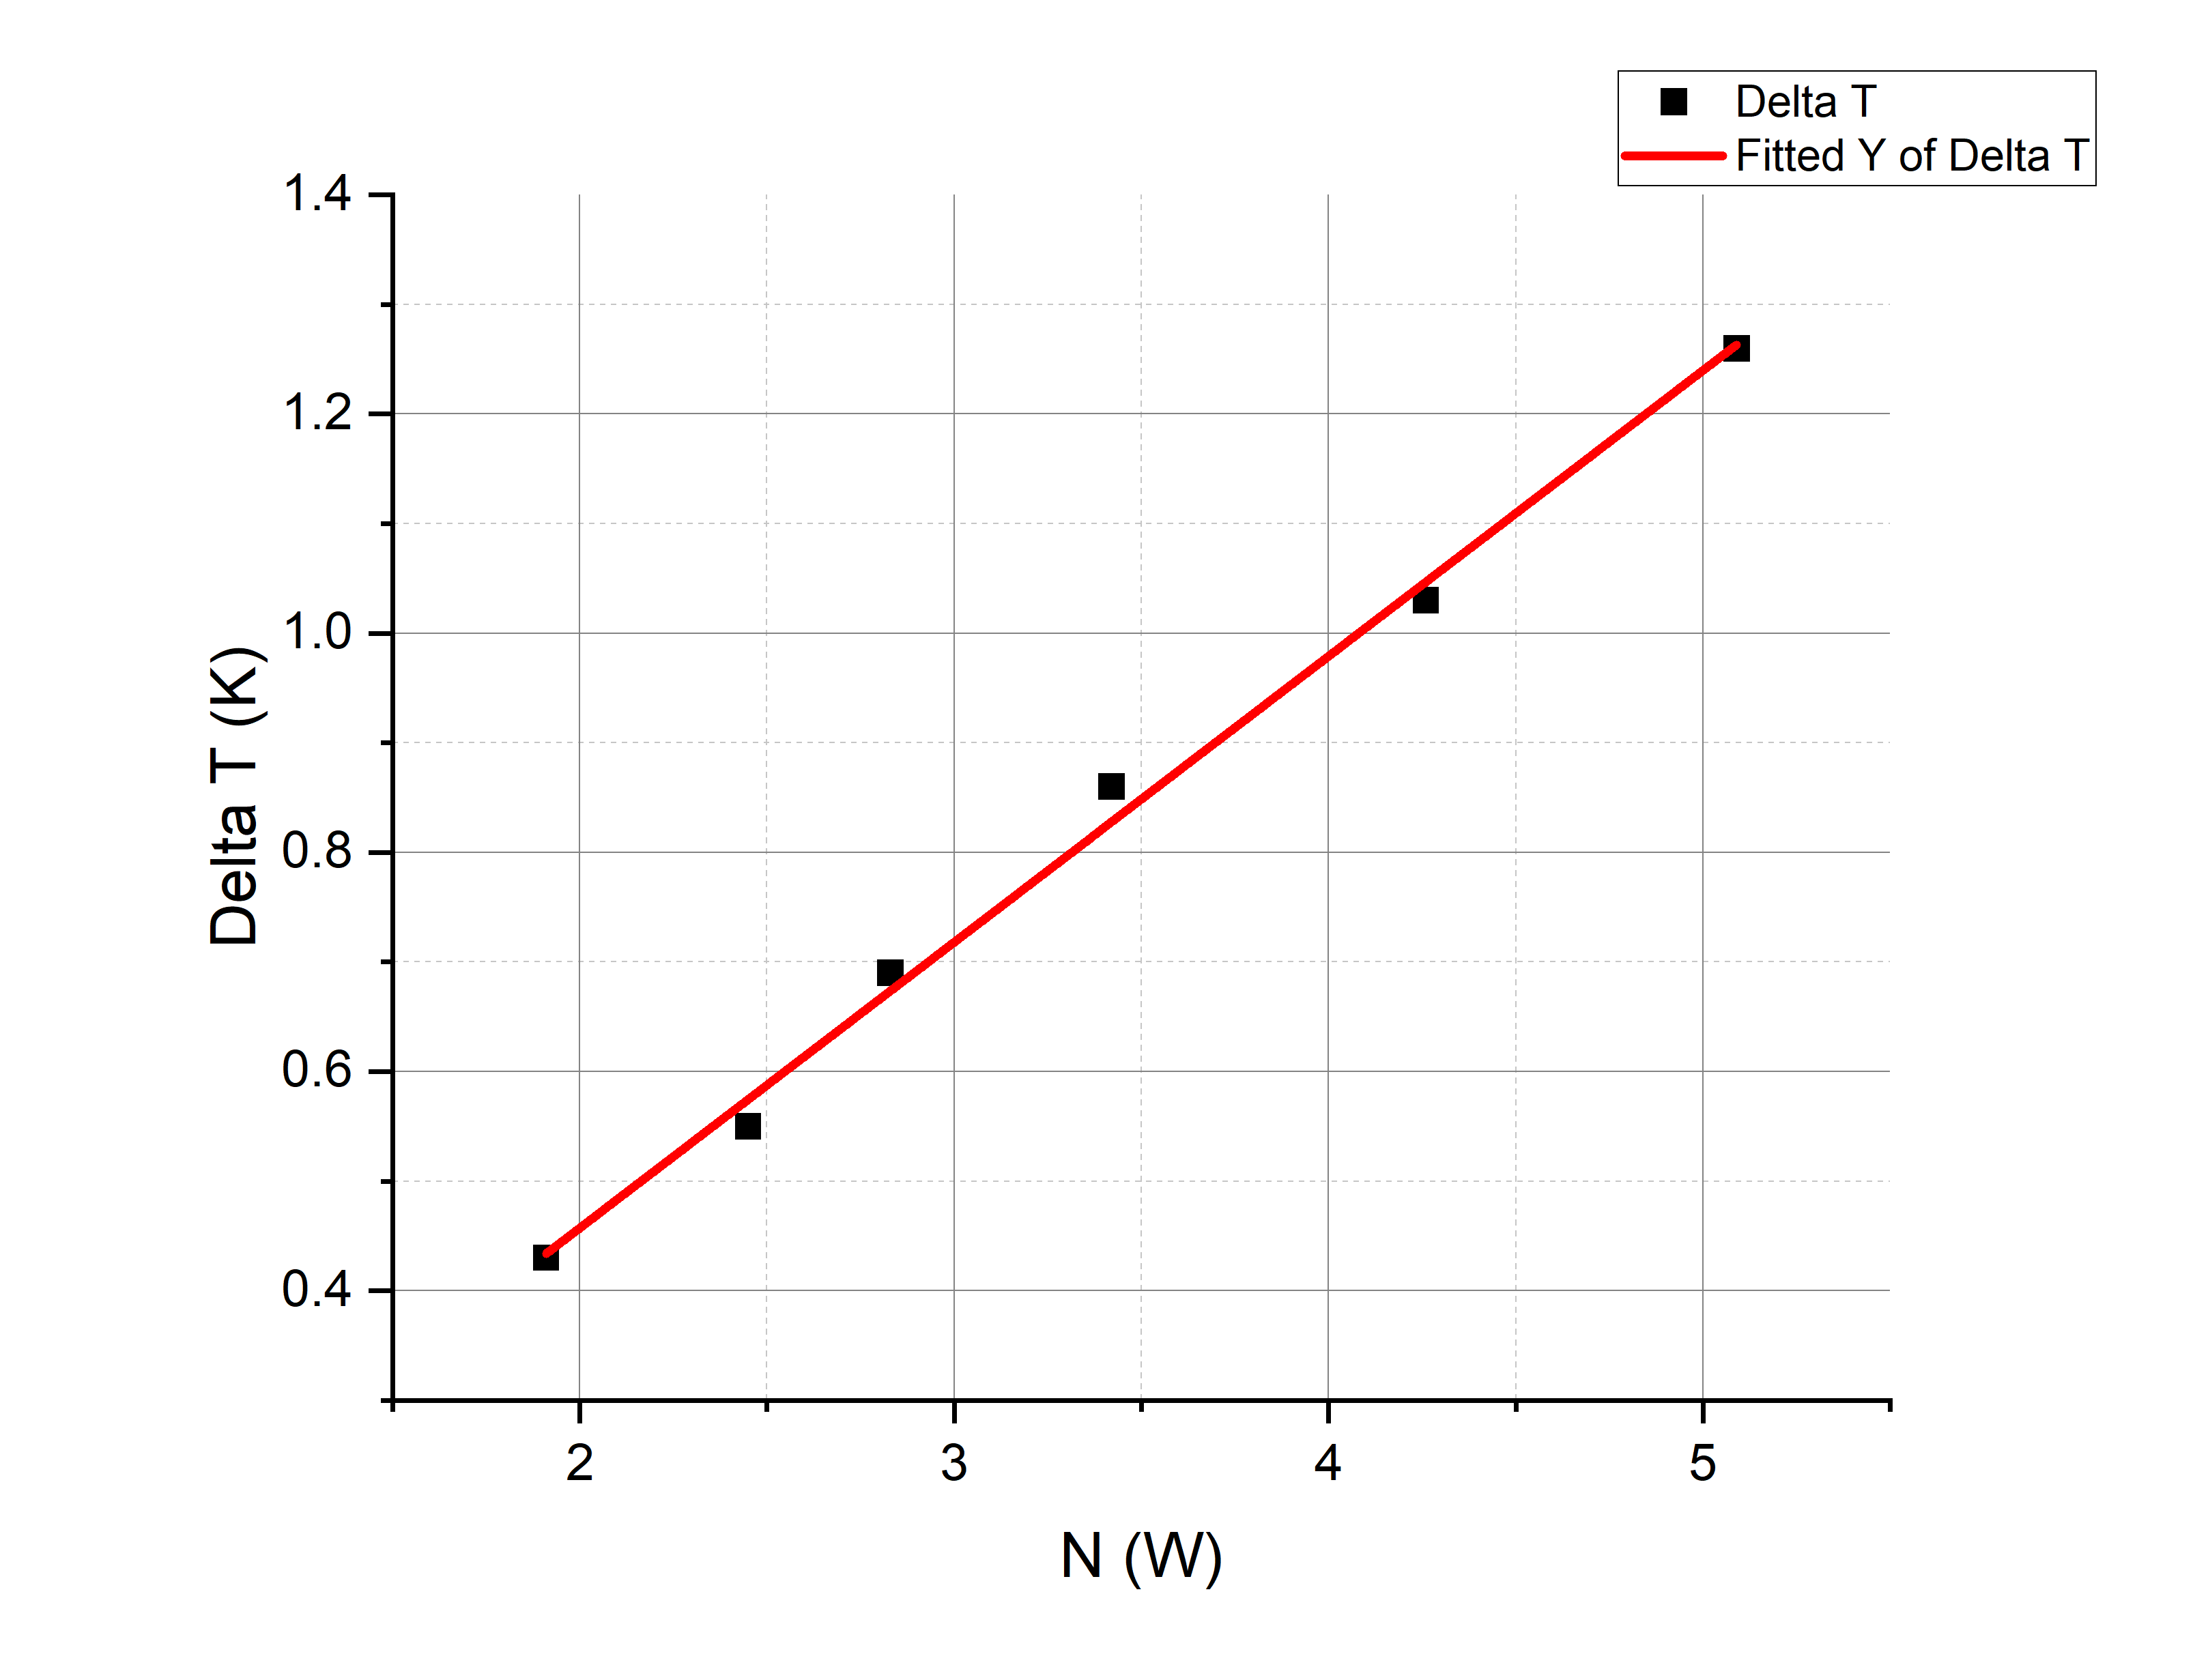
\includegraphics[scale=0.4]{labphoto29.png}
\caption{График зависимости $\Delta T(N)$ при объёмном расходе $q_1$}
\end{figure}

\begin{figure}
\center
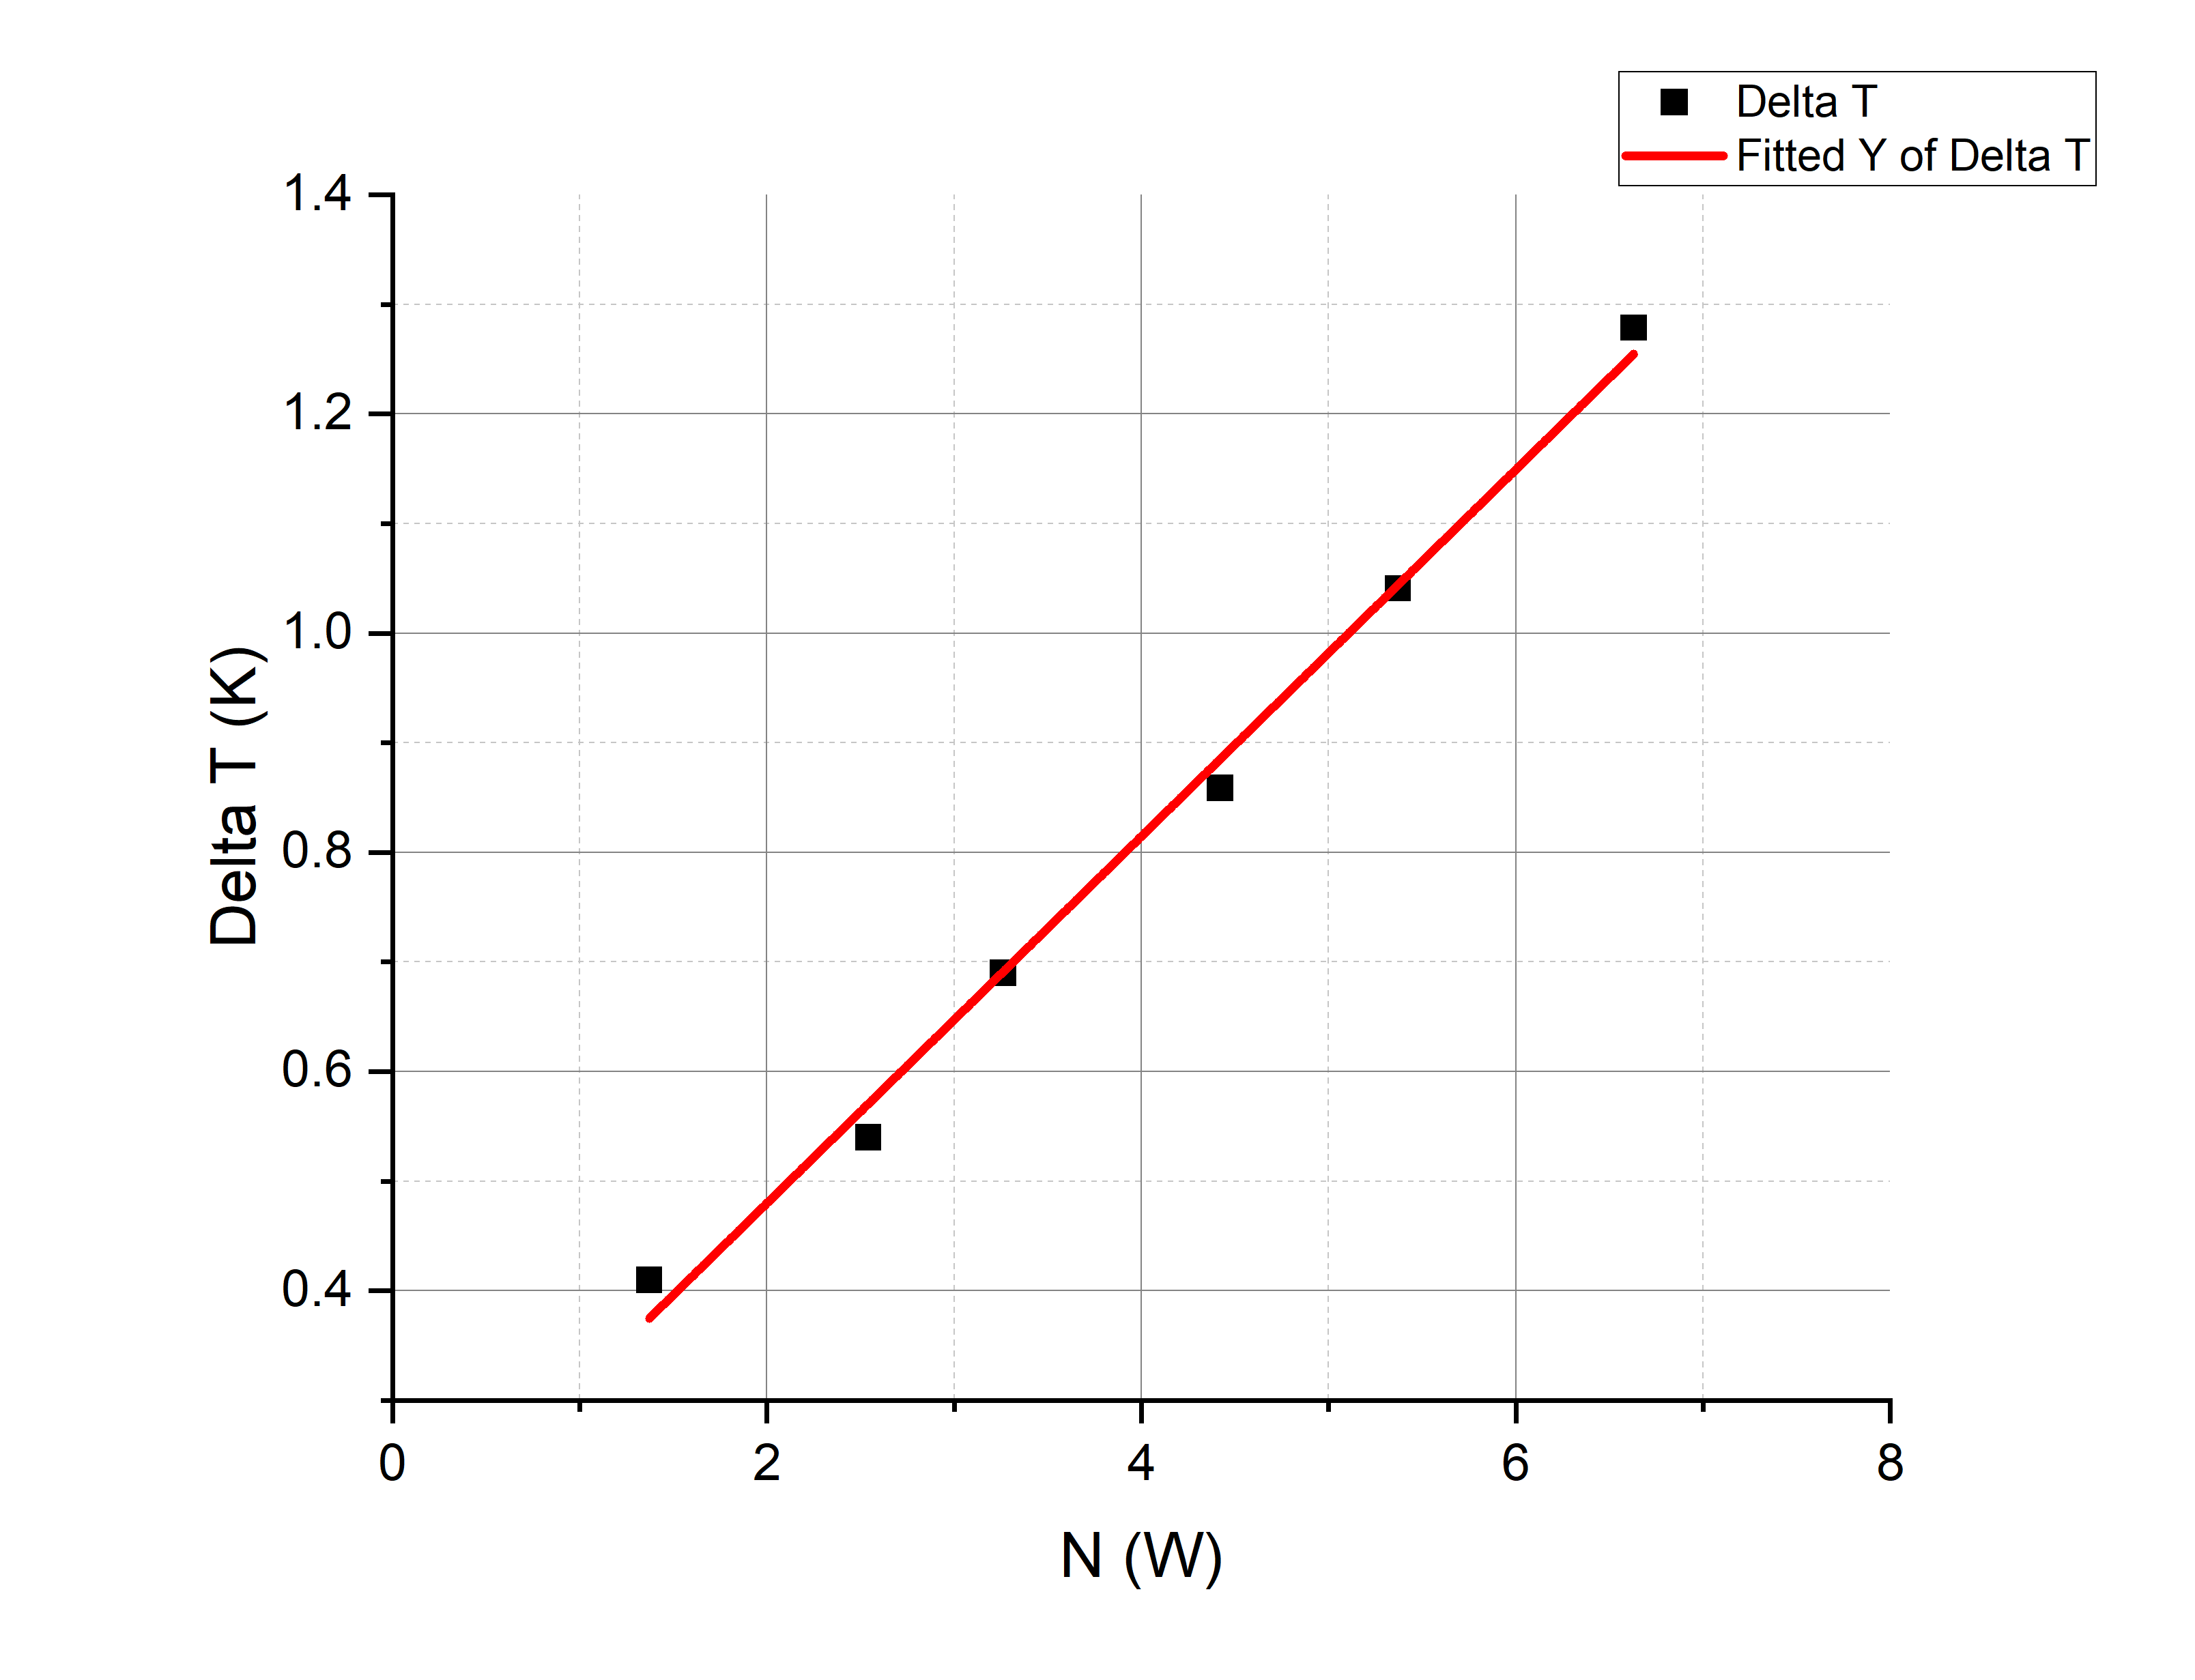
\includegraphics[scale=0.4]{labphoto30.png}
\caption{График зависимости $\Delta T(N)$ при объёмном расходе $q_2$}
\end{figure}
\newpage
Полученные зависиомсти из графиков:
\[
y_1 =k_1 x_1 + b_1;\qquad y_2 = k_2 x_2 + b_2;
\]
\[
k_1 = 3.36 \pm 0.03; \quad b_ 1 = 0.19 \pm 0.04; 
\]
\[ 
k_2 = 4.66 \pm 0.04; \quad b_ 2 = - 0.13 \pm 0.03;
\]
Найдем $\alpha$ и $c_P$, решив систему уравнений:
\[
	\left\{
		\begin{aligned}
			& c_P\, q_1 + \alpha = \frac{1}{k_1} \\
			& c_P\, q_2 + \alpha = \frac{1}{k_2}
		\end{aligned}
	\right.
\]
Путем математических преобразований получаем:
\[
\begin{aligned}
	 c_P = \frac{k_2 - k_1}{(q_1 - q_2)\, k_1\, k_2}; & \qquad  \alpha = \frac{k_2-k_1-c_P(q_1+q_2)}{2\,k_1\,k_2}. \\
	 c_P = 1038\ \frac{\text{Дж}}{\text{кг К}}; & \qquad  \alpha = 0.098\ \frac{\text{Дж}}{K} 
\end{aligned}
\]
Оценим погрешности:

\[
	\sigma_{k_1} = 0.03; \qquad \sigma_{k_1} = 0.04;
\]
\[
	\sigma_{c_P} \approx c_P \sqrt{\left(\frac{\sigma_{k_1}}{k_1}\right)^2 + \left(\frac{\sigma_{k_2}}{k_2}\right)^2} = 13
\]

\[
			\begin{aligned}
			& \fbox{$ c_P  =   1038 \pm 13 \frac{\text{Дж}}{\text{кг К}}$} \\
			& \fbox{$ \alpha = 0.098\pm 0.001\ \frac{\text{Дж}}{K} $}
			\end{aligned}
\]

\section*{Вывод}
Найденное значение молярной темлоёмкости $c_P $ с учётом погрешности и потерь тепла совпадает с табличным значением $c_{P_\text{табл}} = 1003\ \frac{\text{Дж}}{\text{кг К}}$. Мощность потерь тепла в единицу изменения температуры равна $N_\text{пот} = 0.098\ \text{Дж}$.
\end{document}






\end{document}